\def\year{2015}
%File: formatting-instruction.tex
\documentclass[letterpaper]{article}
\usepackage{aaai}
\usepackage{times}
\usepackage{helvet}
\usepackage{courier}
%%
\usepackage{graphicx}
\usepackage{url}
\usepackage{amsfonts}
\usepackage{moreverb}
%%
\usepackage{bm}
\usepackage{paralist}
%%
% so we don't need to specify figures subdirectory in figure code
\graphicspath{{./figures/}}
\usepackage{subfig}

%needed to change table colors
\usepackage[table]{xcolor}
%%
\frenchspacing
\setlength{\pdfpagewidth}{8.5in}
\setlength{\pdfpageheight}{11in}
\pdfinfo{
/Title (Insert Your Title Here)
/Author (Put All Your Authors Here, Separated by Commas)}
\setcounter{secnumdepth}{0}  
 \begin{document}
% The file aaai.sty is the style file for AAAI Press 
% proceedings, working notes, and technical reports.
%
\title{Spoken Dialog Systems for Health Interventions using Fully Autonomous Humanoid Robots}
% \author{{\Large\bf Saminda Abeyruwan} \\ {\Large\bf Andreas Seekircher} \\ {\Large\bf Ubbo Visser}\\
% University of Miami\\
% Department of Computer Science\\
% Coral Gables, FL 33146\\ 
% \{saminda,aseek,visser\}@cs.miami.edu\\
% \And  {\Large\bf Ramesh Baral} \\ {\Large\bf Ugan Yasavur} \\ {\Large\bf Christine Lisetti}\\
% Florida International University\\
% Computing \& Information Sciences\\
% Miami, FL 33199 \\
% \{rbara012,uyasa001,lisetti\}@cis.fiu.edu\\
% }


\maketitle
\begin{abstract}
We integrated a spoken dialog system that we developed to deliver brief health interventions with a 
speech-enabled 3D virtual character with a fully autonomous humanoid robot (NAO). The dialog 
system is based on Markov decision processes (MDPs). We use model free off-policy algorithms in 
reinforcement learning (RL) with the data  collected from real user interactions to obtain the 
(near-) optimal policy. The system begins to learn optimal dialog strategies for initiative 
selection and for the type of confirmations that it uses during the interaction. The health 
intervention framework, delivered by a 3D character instead of the NAO, has already been evaluated, 
with statistically significant results in terms of task completion, ease of use, and future 
intention to use the system.  The current spoken dialog system for the humanoid robot is a novelty 
and exists so far as a proof of concept.
\end{abstract}

%Keywords Spoken dialog Systems á Reinforcement Learning á Virtual Agents and Avatars á Behavior
%Change Brief Intervention

\section{Introduction} \label{intro}

%Spoken dialog systems (SDS) and autonomous humanoid robots are emerging fields of research which, {\em together}, could bring a revolution to human-robot interaction as we know it. 
Latest developments in spoken dialog systems (SDS) show complementary progress for the development of  embodied conversational agents (ECA) \cite{YASCLL14}. Yet, very little of
this progress has been used for autonomous humanoid robots, which have also recently demonstrated the ability
to serve in health interventions. The
humanoid robot NAO specifically has been used in a variety of applications in the health domain (e.g.,
\cite{MAJA13}) including user studies which demonstrate the usefulness of the NAO platform.

Dahl and Boulos (2013) \nocite{robotics3010001} gave a recent overview of how robots are used in
healthcare. Apart from the  surgical robots that are tele-operated by a human doctor, robots support
the daily work in hospitals, mainly in logistics (e.g., Atheon TUG platform \cite{bloss2011mobile}
or HelpMate \cite{evans1998helpmate}). Several other studies have looked at different autism
spectrum disorders. The main goal is to provide therapy with the help of an intelligent robotic
agent that improves both social and communication skills of the children involved. One example is
the KASPAR robot \cite{robins2012scenarios}. Its creators use robot-based play scenarios that can
be tailored for types of disability and skill areas that need to be motivated. Another example has
been created by Bekele and colleagues. They focus on communication behaviors, in particular
head-tracking to manifest the robots engagement in the on-going interaction \cite{bekele2013step}.  

Several studies involve the humanoid robot NAO. Csala and colleagues, for example,
studied the effectiveness of a tele-operated NAO humanoid robot in improving the wellbeing of
children having undergone marrow-transplants. Although there is no conversation with the user
involved, the study demonstrated that the NAO robot is well suited for this task due to its small
size and robustness \cite{Csala2012}. Also, the study identified personalization as a key
requirement for success. The NAO robot has also been used by Belpaeme and colleagues who used the
robot to both entertain and educate children suffering from diabetes in a hospital environment
\cite{belpaeme2012multimodal}. This work is interesting to our approach as it is focused on
providing high levels of robot autonomy using a natural language interface and a long-term memory
structure that allowed children to develop a personal relationship with the robot. Both studies by
Csala and colleagues, and Belpaeme and colleagues, took place in hospitals, and both efforts were
greatly appreciated by the children involved.

Dialog systems can be classified into two main categories based on their dialog management 
technique, which can be either based on machine learning, or hand-crafted.  Systems based on RL are 
popular in the SDS community and are reported to work better than hand-crafted ones for  
speech-enabled systems against noisy speech recognition \cite{young2013pomdp}. 
Hand-crafted systems, on the other hand, can be divided into three subcategories, with dialog 
management approaches using finite states \cite{sutton1998CSLU}, plans and inference rules 
\cite{ferguson1998trips,Bohus2009} or information states. \cite{Traum03}. Intelligent robotics agent 
researchers have not yet integrated these results in their dialog systems to our knowledge. Most 
systems usually involve spoken dialog, and their dialog management usually still relies on 
hand-crafted methods \cite{morbiniFlores2012,Bickmore2010}. 
% BUT BICKMORE AND MORBINI DON'T WORK ON INTELLIGENT ROBOTICS, ONLY 3D CHARS?

In this paper, we discuss a new mode of delivery - a spoken dialog system coupled with a NAO robot - 
for health interventions that can help people adopt healthy lifestyles.  The dialog system can 
deliver brief health interventions (BI), which are short, well structured, one-on-one counseling 
sessions, focused on specific aspects of problematic lifestyle behavior (e.g. overeating, poor diet, 
heavy drinking). BIs, which are top ranked out of 87 treatment styles in terms of efficiency 
\cite{miller2002mesa} and which can be delivered in 3-5 minutes \cite{Moyer2002}, assess a person's 
problem behavior, and provide advice about ways to eliminate it. 


\section*{Approach}

In this section we briefly discuss the approach used to develop the dialog 
agent (see \cite{YASCLL14} for more details). According to the 
clinician's guide for conducting brief interventions from the National Institute on Alcohol Abuse 
and Alcoholism (NIAAA) \cite{national2007helping}, a brief intervention for alcohol-related health 
problems can be delivered in three sequential steps (Figure 
\ref{fig:dialog_manager}): \begin{inparaenum}[1)] \item {\em Screening} about alcohol use; \item 
{\em Assessing} for alcohol use disorders in two sequential processes: \begin{inparaenum}[a)] \item 
assessment of potential alcohol {\em abuse}; and \item assessment  of potential alcohol {\em 
dependence}\end{inparaenum}; \item {\em Advising} and assisting the patient according to 
the degree of alcohol problems which leads to: \begin{inparaenum} \item advice for {\em at-risk} 
drinkers; \item and advice for drinkers with alcohol use {\em disorder} (e.g. coordinate care with specialist). \end{inparaenum} 
\end{inparaenum}

\subsection*{Dialog Structure for Brief Interventions}

The development of the brief intervention content is based on the guide provided by 
NIAAA \cite{national2006niaaa}. The goal of the dialog agent is to deliver alcohol screening and 
brief interventions based on this guide. Each step contains a set of questions. The screening for heavy drinking step 
uses 5 questions to access the user's {\em alcohol use} or consumption.  If the user 
expresses that (s)he is not consuming alcohol from time to time, the interaction is  ended gracefully
 with advice on recommended limits, otherwise, the dialog continues to the {\em alcohol use disorders} assessing step.  

The {\em assessment of alcohol use disorder (abuse or dependence)} step consists of two sequential processes: \begin{inparaenum}[1)] \item the 
{\em assessment of alcohol abuse} sub-step, where, there are 4 questions to assess alcohol abuse indicators.  It is 
enough to find one indicator of alcohol abuse (e.g., risk of bodily harm, relationship trouble) to 
move to \item the {\em assessment of alcohol dependence} step   (e.g., keep drinking despite problems, not able 
to stick to drinking limits). If the system can not find any indicator of abuse with the 4 
questions, it passes to the {\em assessment of alcohol dependence} sub-step, which has  7 questions to access the user's state. 
\end{inparaenum}

It is enough to detect 3 dependence indicators to transit to the step {\em advice on alcohol use disorder (abuse or dependence)}.  If the system does not detects 3 dependence 
indicators, it transits to {\em advice for at-risk drinking}. Therefore, the dialog branches to two 
separate steps at the end of the assessment of alcohol use disorder step. In both branches, the system provides information 
related to the assessment of the system.  If the system assessed that the user has an {\em alcohol use 
disorder}, it refers the user to treatment, e.g. refer to an addiction specialist, suggests a drinking goal.  If 
the system assessed that the user is an {\em at-risk drinker}, it gauges his or her readiness to change, and provides feedback and 
information about the person's drinking. Therefore in both stages, the system provides factual 
information about the person's drinking and suggested drinking limits, and asks what is the user's 
intention to change with a single question.  In total there can be a maximum of 18 different 
questions in a complete session.   

\begin{figure}[!t] 
\centering 
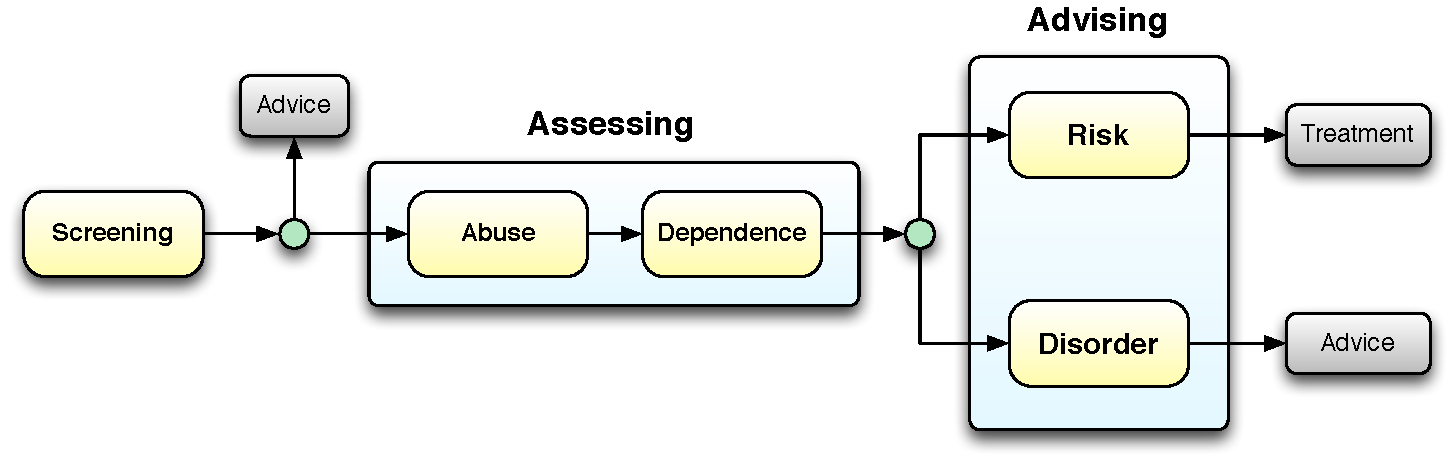
\includegraphics[width=.45\textwidth]{figures/dialog_manager_v2} 
\caption{Dialog structure for brief interventions.} 
\label{fig:dialog_manager} 
\end{figure}

\subsection*{Dialog Agent with Reinforcement Learning}

The goal of the dialog system is to find a (near-) optimal policy that guides the user to an advice 
or a treatment appropriate to the user's alcohol use (the grey boxes in Figure \ref{fig:dialog_manager}) in an efficient manner. 
Model free off-policy algorithms in RL (e.g., Q($\lambda)$ \cite{sutton1998reinforcement}, 
Greedy-GQ($\lambda$) \cite{maei2010toward}, off policy actor-critic \cite{DegrisWS12}) provide the 
means to find (near-) optimal dialog policies by having the agent learn them 
from real experiences, and reward feedbacks. In addition, the RL framework provides many advantages over hand-crafted approaches \cite{lemon2007machine}: \begin{inparaenum}[1)] \item a 
data-driven automatic development cycle; \item provably optimal or near-optimal dialog policies; 
\item  a principled mathematical model for action selection; \item  possibilities for generalization 
to unseen states; and \item reduced development and deployment costs.\end{inparaenum} 

The RL framework is an generalization of MDPs \cite{sutton1998reinforcement}. In oder to develop an RL 
agent, the designer provides the descriptions of the states, actions, and reward functions. As the 
first step, to avoid the data sparsity problem during learning, the whole system has been 
divided into 5 RL problems (the yellow boxes in Figure \ref{fig:dialog_manager}) and learned their 
(near-) optimal policies independently. 
%DON'T FOLLOW THIS SENTENCE, DO YOU MEAN 'AND LEARNS..."?. 

A {\em state} is described with 5 features with discrete values: \begin{inparaenum}[1)] \item type of question (open or closed); 
\item confidence (of speech recognition); \item value; \item grammar; and \item auxiliary. \end{inparaenum} Each 
question is mapped to a possible state. According to our definitions, each question will produce 34 
potential states (some associated states per question have been pruned due to non-reachability). 
Therefore, the dialog agent uses a total of 578 states to represent the states of the environment. Each 
state is associated with 2 actions based on initiative and  confirmation types. The reward 
function is designed to complete each RL problem with the minimum possible number of steps (see \cite{YASCLL14} for details).  

A rich dialog corpus was used during the learning process. The corpus is organized turn by 
turn. Each turn element contains: stage and state information, question asked by the system,  
initiative type,  best speech recognition, grammar type, semantic value or result of the semantic 
parser, N-best recognitions with confidence score, reward gained from the question, cumulative 
reward and sound files. Each XML log file contains sequences of dialog turns for one dialog 
session (Table \ref{sampleDialog} shows  sample dialogs for each stage). The off-policy model free 
Q($\lambda$) algorithm has been used to learn a (near-) optimal policy.

\begin{table}[!h]
\caption{Sample Dialogs for each Intervention Step}
\label{sampleDialog}
\begin{tabular}{ p{80mm}  } \hline
    \textbf{Asking about Alcohol Use} \\
    Hello, my name is Doctor House. I am a humanoid robot created to have conversations about 
healthy lifestyle. Today, I am here to talk about drinking to figure out if you have any issues.  
May I ask you few questions about your drinking? \\
\bf{\em{Yes, sure you can.}}\\
Do you sometimes drink beer, wine, or other alcoholic beverages?\\
\bf{\em{Well yes, I drink wine or beer sometimes!}} \\
$\ldots$\\
Ok, thanks for the information you have provided to me about your drinking. Next, I will try to 
determine some important effects of your drinking. \\
    \hline
    \textbf{Assessing for Alcohol Use Disorders} \\
    Have you ever taken risks under the influence, such as drinking and driving, operating a motor 
vehicle, or swimming?\\
\bf{\em{No I have not.}} \\
I see, so you are careful to avoid high risk situations after or while having drinks, right?\\
\bf{\em{Yes, I try to be careful.}} \\
$\ldots$\\
Have you had a period when you spent a lot of time drinking? Or being sick or getting over the bad 
aftereffects of drinking? \\
\bf{\em{Yes several times.}} \\
    \hline
    \textbf{Advising} \\
     Thank you very much for all your answers. Now I'd like to just take one or two more minutes of 
your time. Is that okay? \\
\bf{\em{Yes, please go ahead.}}\\
$\ldots$\\
Thanks for talking with me. I hope you've learned something useful about your drinking pattern.  
Good bye and let's talk again in 3 months! \\
    \hline
\end{tabular}
\end{table}


\section*{Implementation} 

Our implementation is based on two system designs that were independently
invented and developed in two different research groups. The FIU Affective Social Computing group developed a dialog manager integrated with a 3D virtual 
character.  Our system utilizes the user's natural speech as one input parameter and also uses gaze
and non-verbal cues for the classification of the user's state. The dialog manager (successfully tested with 87 users) operates with five
interconnected MDPs, each representing a step of the intervention \cite{YASCLL14}. The dialog 
manager uses domain specific dialog phrases, with a tailored semantic parser, and a RL agent that 
learns over time how to address/answer the user. 

\begin{figure}[!t] 
\centering 
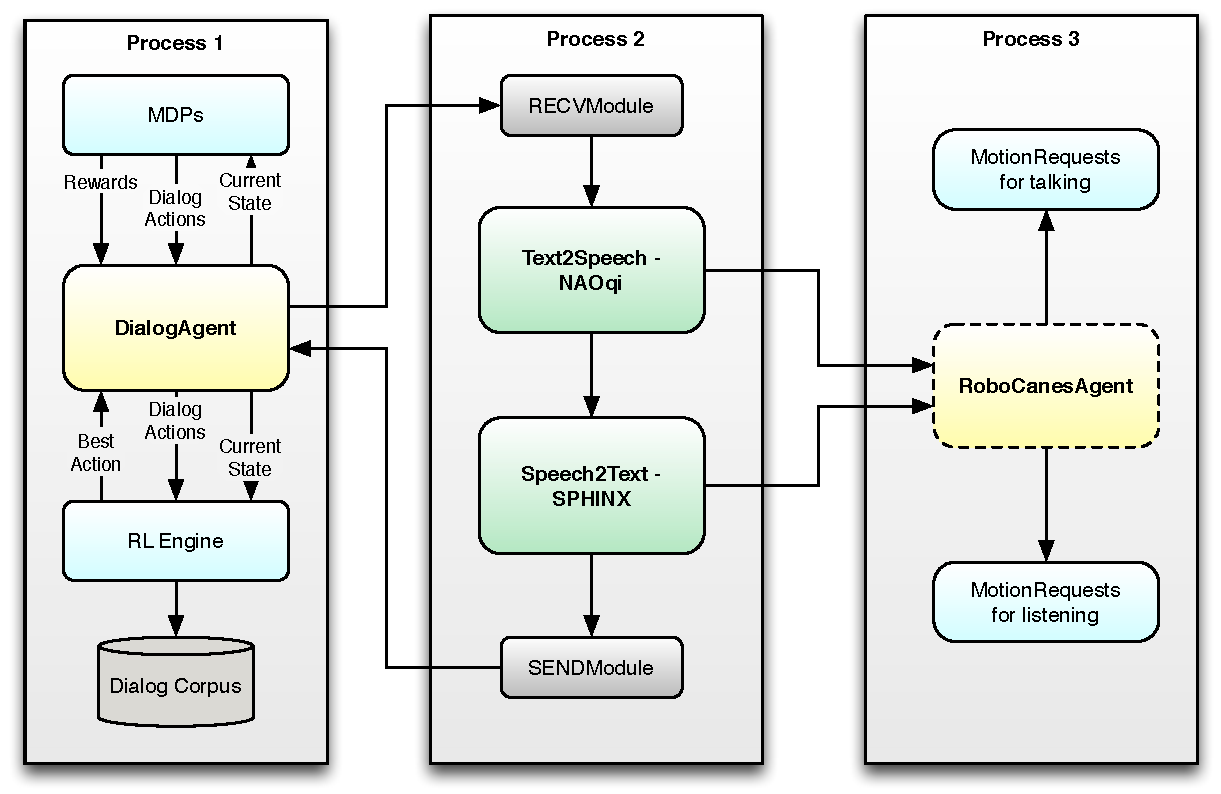
\includegraphics[width=.46\textwidth]{figures/system} 
\caption{System Architecture: {\em Process 1} is the dialog manager; {\em Process 2} delivers the 
robot's spoken utterances and the recognized human's utterances; and {\em Process 3} senses the 
human's non-verbal cues, and controls the robot's motions for appropriate gestures during the 
robot's speech and listening time (e.g. tracks user's face and, if user moves, moves to maintain 
facing position.)} 
\label{fig:system} 
\end{figure}


The University of Miami's autonomous robots research group develops methods for both simulated and
physical agents that act in dynamic, adversarial, and real-time environments. 
%The group uses the RoboCup domain as an area of investigation. 
One  focus is the consideration of agent's
actions/behavior to make its own decisions 
%(for the own team agents). 
The group has developed a fully implemented system (RoboCanes software) using six NAO robots that not only move in the
mentioned environment on their own, but also have to consider team communication (e.g. for global
object positions such as the ball or an opponent agent) and cooperation. The software is stable and
robust and is used as part of the backbone for this research paper.

We ported the dialog manager on one of our NAO robots. The software runs as a single process. The
dialog manager is connected to another process on the robot that makes use of Google speech API 
version 2. The original dialog system described in \cite{YASCLL14} has a language model and 
grammars, which we plan to  adapt for the NAO robot in our next system version. A third process is 
the RoboCanes software that can be connected to the dialog. Figure \ref{fig:system} gives an 
overview of the architecture and the three processes. Process 1 is connected to process 2 using 
Java JNI interface. The robot receives a greeting mechanism  at the beginning of a conversation that 
can be altered when starting again. The NAO robot then uses NAOqi for the Text-To-Speech 
generation, although we have also implemented and tested other systems such as Festival 
\cite{taylor1998architecture} or eSpeak \cite{eSpeak}, which would also work. Process 2 then makes 
use of the RoboCanes framework (the RoboCup agent) which is responsible for robot motions and also 
for the image processing and the audio feedback (no feedback from cameras at the moment yet). The 
robot then uses Google speech API, turns the audio signal into text and sends it back to the dialog 
manager. The timing between processes 1 and 2 are based on turns, process 3 runs with 100 Hz for the 
joint requests and 30 Hz for both cameras.

\section*{Conclusions} 

Although currently at the prototype stage, we anticipate that the NAO robot will become a very 
likable and effective mode of delivery for brief interventions for target behaviors such as poor 
diet, overeating, or lack of exercise, among others.  The appeal of the NAO to children 
\cite{belpaeme2012multimodal} makes it particularly suitable to become a child's favorite health 
coach, say, to discuss eating more fruits and vegetables on a daily basis. Our platform 
provides the additional advantages such as a dialog system for a lack of exercise or  it can 
also demonstrate physical exercises.

\bibliographystyle{aaai}       
\bibliography{library}   


\end{document}
